

\begin{frame}{\ft{The Photo Viewer}}

\doubleFrame{Re-PDF provides a suite of useful dialog boxes 
and a toolkit for programming customized presentations according 
to the preferences of each realtor.  For example, one 
standard format would be a color-coded property-photo viewer with 
thumbnail-sized previews of each image.  The whole set of 
thumbnail photos can then be seen together 
alongside the larger photo being viewed, rather than 
users having to scroll between groups of four 
or five thumbnails at a time.  
Users can enlarge photos by clicking on 
their thumbnails, or view photos in 
sequence via left/right arrows.}

\vspace{-1em}
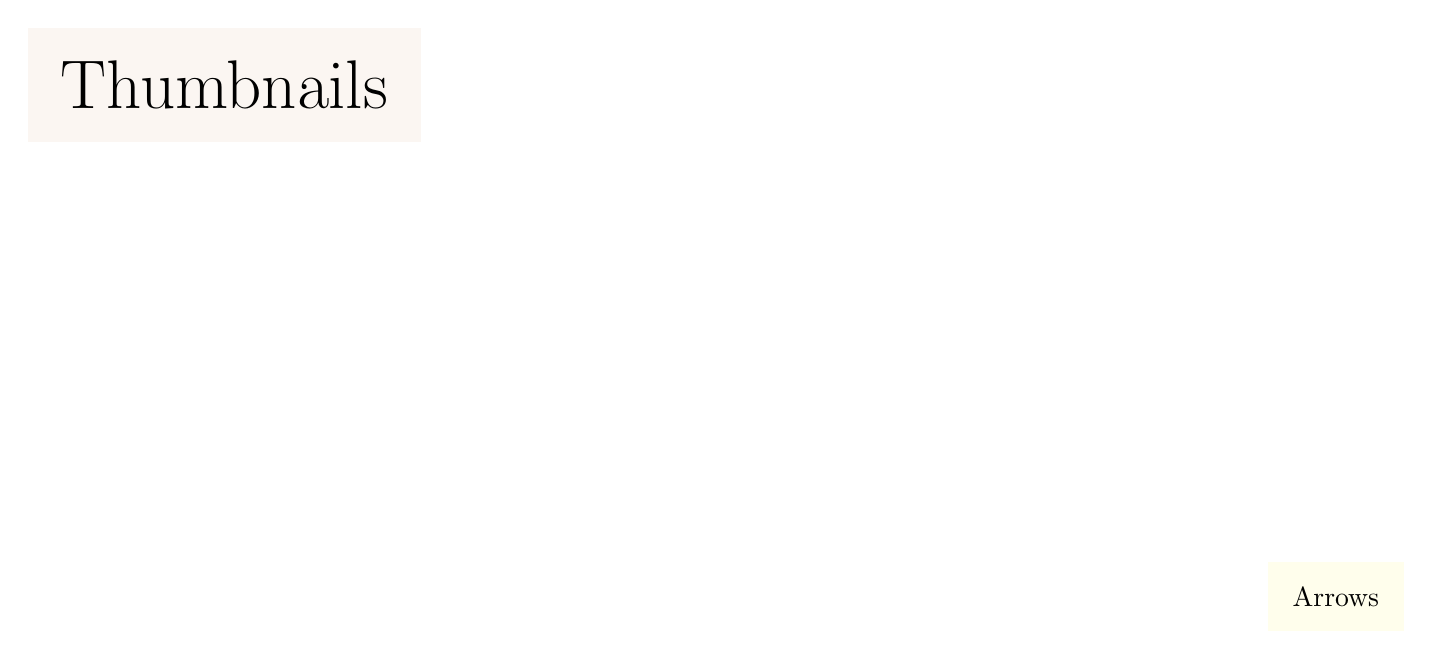
\begin{tikzpicture}
%\nodeincludegraphics[0.89\textwidth]{screenshots/ss-ph1.png}
\nodeincludegraphicsTRRS{1}{3.3cm}{3cm}{2cm}{1cm}{screenshots/ss-ph1.png}

\ann{BlueGreen}{0.3}{1mm}{grammarArrowColor}{0.5}{13.5,8}{5}{4.5}{0.95}

%\node [anchor=west] (note) at (6.25,9) {\Huge {\color{blGreen!30!black}Thumbnails}};
\node [anchor=west,fill=brown!8!white,inner sep=12, 
opacity=0.88, text opacity=1] (note) at (2.95,9.1) {\Huge {\hc{Thumbnails}}};

\colorarr{>=latex, ->}{fcBoxColor!60!black}{0.8}%
{blGreen!30!red}{1}{1mm}{[xshift=2em,yshift=.4em]note.south}{8.5, 8}

%\node [anchor=west] (noteArr) at (20.15,3) {\Huge {\color{blGreen!30!black}Arrows}};

\node [anchor=west,fill=yellow!15!white,inner sep=9, 
opacity=0.5, text opacity=1] (noteArr) at (18.7,2.6) {\hc{Arrows}};


\colorarr{>=latex, ->}{fcBoxColor!60!black}{0.8}%
{blGreen!30!red}{1}{1mm}{noteArr.south}{20.15,1}

\end{tikzpicture}


\end{frame}

